
\LoadClass[12pt,letterpaper]{article}
\RequirePackage{palatino}
\RequirePackage{verbatim}
\RequirePackage{amsmath,amsfonts,amsthm,amssymb,multirow,xcolor}
\RequirePackage{geometry}
\RequirePackage{graphicx}
\RequirePackage{datetime2}
%===================================================
\renewcommand{\maketitle}{
\hrule height 1pt
\begin{center}
{\bf \large Proposal}\\[2mm]
{Jiachun Zhang}\\[2mm]
{\today}\\
\end{center}
\hrule height 1pt
}
\graphicspath{ {./images/} }
%===================================================
\geometry{left=1in,right=1in,top=1in,bottom=1in}
\begin{document}
\maketitle
\section*{Introduction}
Current standards for music information retrieval (MIR) are based on the 
12 tone equal temperament (ET) scale (midi, musicxml, etc.). However, when 
they are being used in the context of tonal music, a lot of problem arises.
For example, the notion of \textit{scale degree} and \textit{key signature} is lost in the ET.
However, notations used in tonal music can be very hard to parse and implemented in 
digital communication sytems. Take diatonic harmony for example, the conventional major
and minor keys can be recognized easily by human musicians with correct notations in 
a 5-line staff because of the key signature notation. But it is very hard to implement 
into a digital system that requires a lot of hommogeneous data that is generalized 
to be used in various situations. This research will focus on a new way to represent 
tonal music suitable for vectorizationa and digital communication. The final goal is to come 
up with a new way to represent music with implicitly embedded tonal/atonal information by looking 
into previous proposed methods.
Topic to be covered would be:
\begin{itemize}
\item Algorithms for determining the key of a piece.
\item Various metrics/procedures of determining the "fitness" of a genre such as fugue, sonata given a music piece.
\item Algorithms that projects current discrete music data into a continuous space with implied 
tonal/atonal information.
\end{itemize}

\section*{Transposition}
Let us first look at a simple operation in tonal music -- Transposition. Transpositon moves a 
collection of notes by certain interval. It is very common in classical music the opening
statement is transposed to the dominant key. We shall
write a very simple melody in the key of C:

\begin{center}
    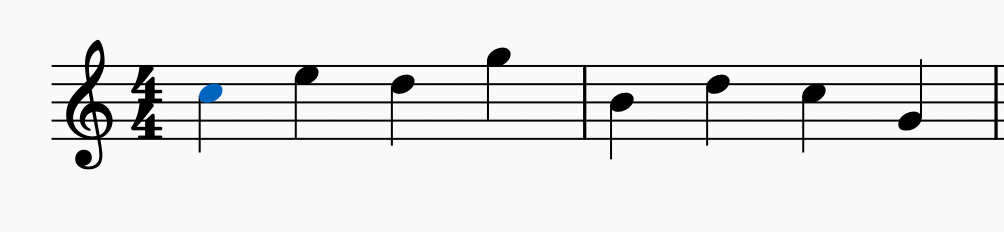
\includegraphics{1}
\end{center}

We can write these notes in a vector form $[0, 4, 2, 7, 11, 2, 0, 7]$. The phrase
starts with C and ends in G. Transpose it strickly to its dominant key, G, we get:
\begin{center}
    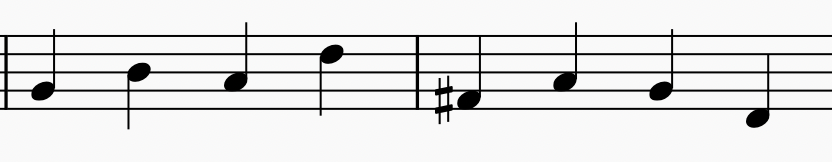
\includegraphics{2}
\end{center}
The second phrase is now in the key of G. We can write it in vector 
form $[7, 11, 9, 2, 6, 9, 7, 2]$. We know it is an element in the T7 group,
which transpose everything up by 7 or down by 5 semitones. But sometimes 
the phrase can be twicked a little bit to make it more interesting. For example,
the second phrase can be written as follows:
\begin{center}
    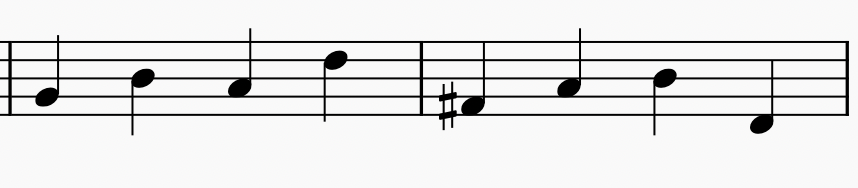
\includegraphics{3}
\end{center}
G in the second bar now becomes B, are they still similar in some way? 
We as humans can tell they are similar by ear easily, but how can we show they are 
similar by numbers? One possible way we can do is to calculate their "cosine similarity". 
We shall calculate differences between first and 2 other phrases, whcih can written as $u, v$:
\[[7,7,7,7,7,7,7,7], [7,7,7,7,7,7,11,7]\] and then calculate the cosine similarity between them:
$\cos(u, v) = \frac{u\cdot v}{|u|\cdot |v|}\approx0.98$.\\
This is just one method of looking at melodic similarity, which might be not acurate since
it does not consider the potential harmoic information implied by the melody, or base 
accompanied. Nevertheless, it should be a new way to look at how we can interpret music
in another way.

\section*{Conclusion}
More questions raise as we take more things into consideration, such as how to find a 
algorithm that can look at their harmonic similarity which might imply some aspect of 
tonal funtion analysis. It would be a multiple step process to reach to the final solution,
we shall first start with a problem with smaller goal, such as finding the key of a piece
with the current 12 time representation of music. Then we can move on to a higher level 
problem.

\end{document}

